\documentclass[aspectratio=169]{beamer}
\usetheme[block=fill]{metropolis}
\usepackage{tikz}
\usetikzlibrary{shapes.geometric, arrows.meta, positioning, calc}

\title{Building a Reproducible Scholarly Search Toolkit}
\subtitle{Episode 12: The Provider Protocol \& In-Memory Engine}
\author{Scholar Search Kit}
\date{}

\begin{document}

\begin{frame}[plain]
  \titlepage
\end{frame}

\begin{frame}{Episode Goal}
  \begin{alertblock}{The Goal}
    Define a \texttt{SearchProvider} Protocol and implement an \texttt{InMemoryProvider} for blazing-fast, network-free testing.
  \end{alertblock}
  \vspace{0.5cm}
  If our unit tests actually hit the OpenAlex API, they will be slow, flaky, and require internet access. We need a way to completely mock the provider layer.
\end{frame}

\begin{frame}{The \texttt{SearchProvider} Protocol}
  \begin{center}
  \resizebox{0.5\linewidth}{!}{
  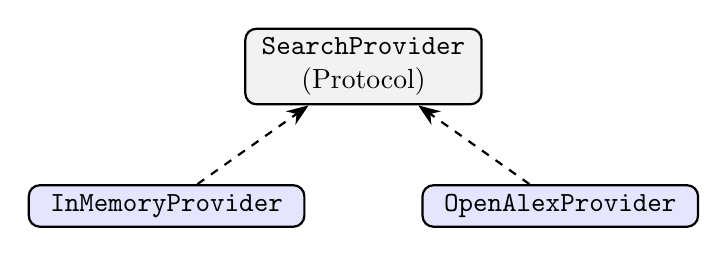
\begin{tikzpicture}[
      node distance=1.5cm and 2cm,
      proto/.style={rectangle, draw, thick, rounded corners, minimum width=3cm, align=center, fill=black!5},
      impl/.style={rectangle, draw, thick, rounded corners, minimum width=3.5cm, align=center, fill=blue!10},
      arrow/.style={-{Stealth[scale=1.2]}, thick, dashed}
    ]
    
    \node[proto] (p) {\texttt{SearchProvider}\\(Protocol)};
    
    \node[impl, below=1cm of p, xshift=-2.5cm] (mem) {\texttt{InMemoryProvider}};
    \node[impl, below=1cm of p, xshift=2.5cm] (oa) {\texttt{OpenAlexProvider}};
    
    \draw[arrow] (mem) -- (p);
    \draw[arrow] (oa) -- (p);
  \end{tikzpicture}
  }
  \end{center}
  \vspace{0.2cm}
  Any class that implements \texttt{search(query: Query) -> SearchResult} satisfies the Protocol.
\end{frame}

\begin{frame}{Implementation: \texttt{InMemoryProvider}}
  \begin{block}{Deterministic Testing}
    The \texttt{InMemoryProvider} is initialized with a static list of \texttt{Document} objects.
  \end{block}
  
  \begin{itemize}
      \item When \texttt{search()} is called, it simulates latency and returns the predefined list.
      \item This allows the rest of the application (deduplication, export, CLI) to be tested instantly without network variability.
  \end{itemize}
\end{frame}

\begin{frame}{The Registry Pattern}
  \begin{block}{Dynamic Injection}
    We use a \texttt{ProviderRegistry} to map names (e.g., "openalex") to their respective classes.
  \end{block}
  
  \begin{itemize}
      \item The CLI doesn't need to import \texttt{OpenAlexProvider} directly.
      \item This allows users to pass \texttt{--provider=openalex} and instantiate the engine dynamically.
  \end{itemize}
\end{frame}

\begin{frame}{Verification}
  \begin{alertblock}{Success Criteria}
    \begin{itemize}
        \item The \texttt{InMemoryProvider} successfully passes the Pyright type-checker as a \texttt{SearchProvider}.
        \item Fetching "in\_memory" from the \texttt{ProviderRegistry} returns the correct class.
    \end{itemize}
  \end{alertblock}
\end{frame}

\end{document}
